\chapter[Planejamento do projeto]{Planejamento do projeto}

  \section{Cronograma}
  
   O cronograma do projeto foi dividido em duas fases principais, a fase de iniciação/planejamento, onde será elaborado o planejamento
   necessário para a execução do projeto, e a fase de execução, onde será executado todo o planejamento.
   As figuras ~\ref{cronograma_1}, ~\ref{cronograma_2}, ~\ref{cronograma_3} e ~\ref{cronograma_4} ilustram o cronograma do projeto.
   \vfill
  
  \pagebreak
  \begin{figure}[!htbp]
    \centering
    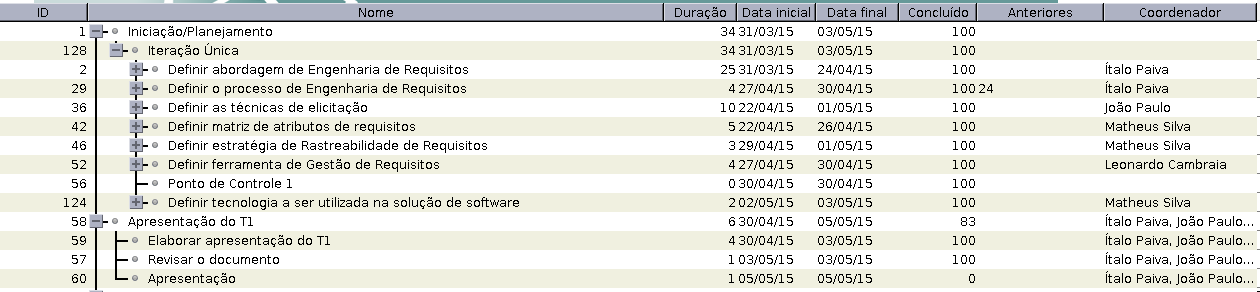
\includegraphics[scale=0.5, angle = 90]{editaveis/figuras/cronograma_1}
    \caption[Cronograma - Fase de Iniciação]{Cronograma do projeto - Fase de Iniciação.}
    \label{cronograma_1}
  \end{figure}
  
  \pagebreak
  \begin{figure}[!htbp]
    \centering
    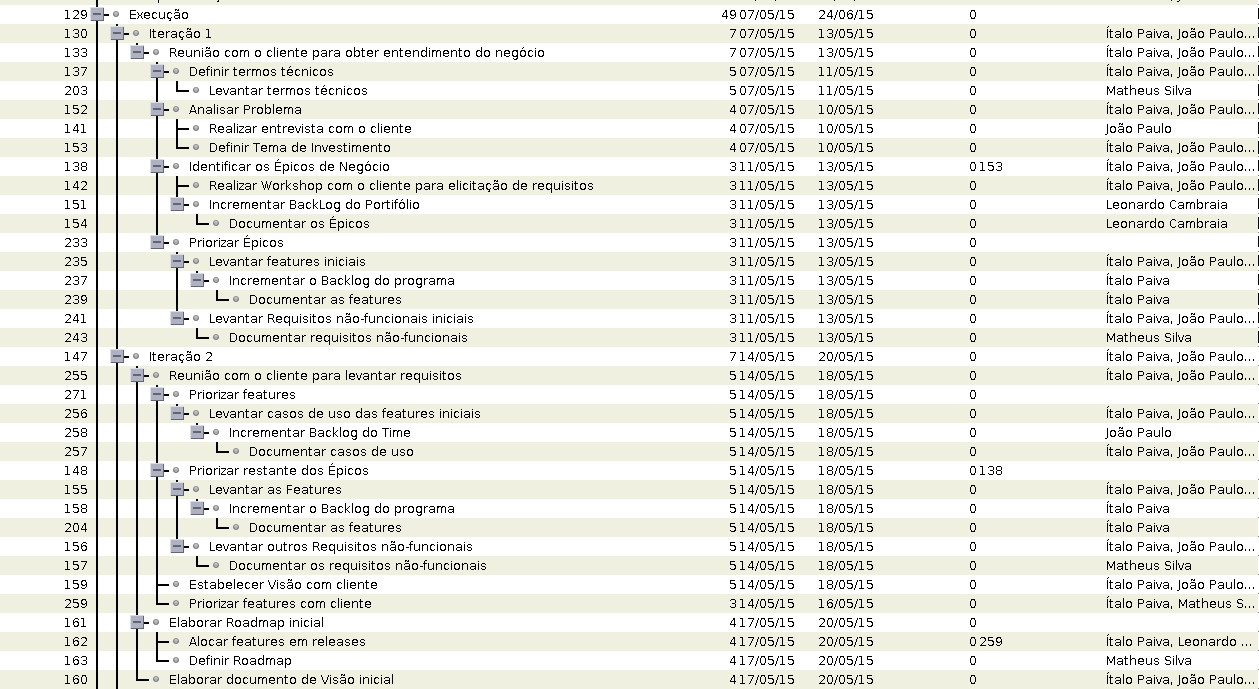
\includegraphics[scale=0.5, angle = 90]{editaveis/figuras/cronograma_2}
    \caption[Cronograma - Fase de Execução]{Cronograma do projeto - Fase de Execução até a iteração 2.}
    \label{cronograma_2}
  \end{figure}
  
  \pagebreak
  \begin{figure}[!htbp]
    \centering
    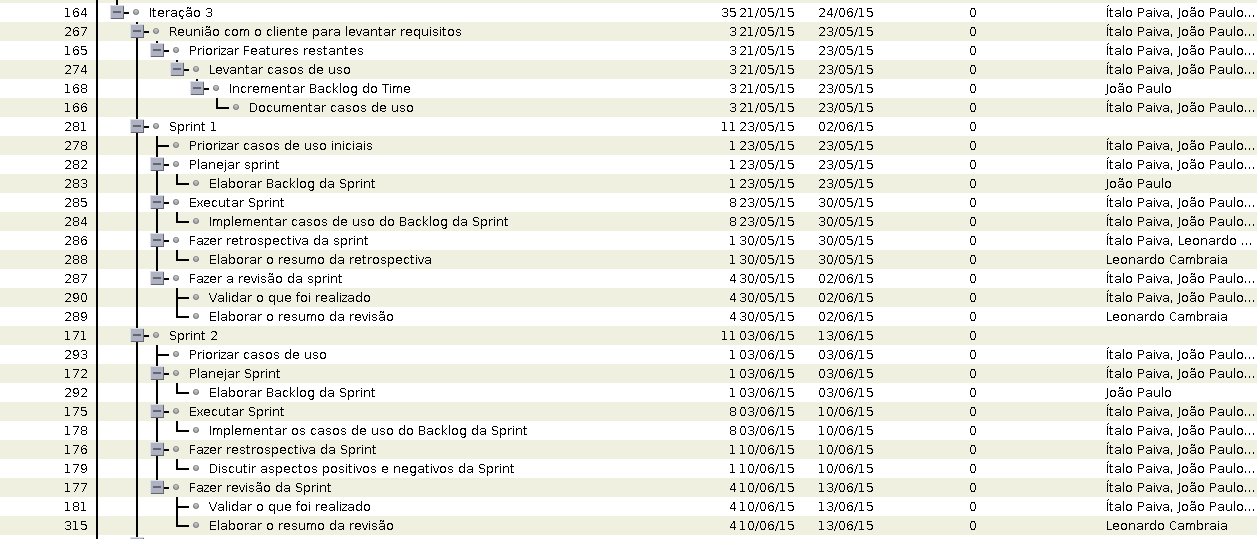
\includegraphics[scale=0.5, angle = 90]{editaveis/figuras/cronograma_3}
    \caption[Cronograma - Fase de Execução]{Cronograma do projeto - Fase de Execução até a iteração 3, \textit{sprint} 2.}
    \label{cronograma_3}
  \end{figure}
  
  \pagebreak
  \begin{figure}[!htbp]
    \centering
    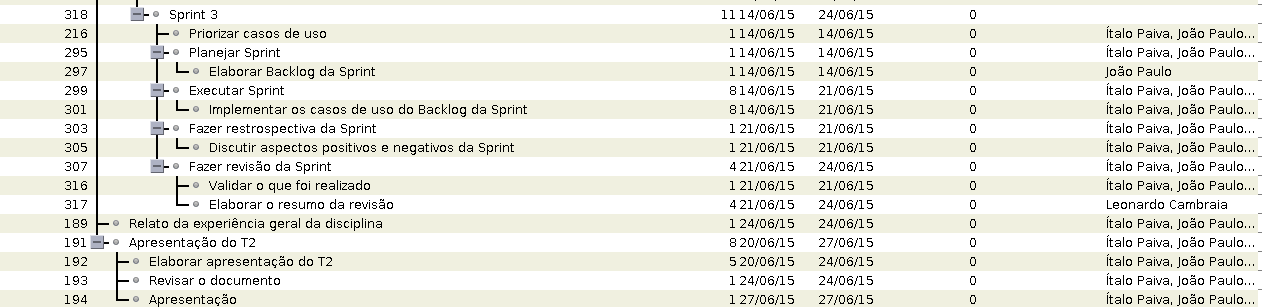
\includegraphics[scale=0.5, angle = 90]{editaveis/figuras/cronograma_4}
    \caption[Cronograma - Fase de Finalização]{Cronograma do projeto - Fase final e \textit{sprint} 3.}
    \label{cronograma_4}
  \end{figure}